\chapter{Introduction}\label{chap:01}
\begin{chapter-abstract}
Here I give an overview on my thesis.
This includes general topic and field of research (perceptual quality judgment that relies on memorization and then recall).
I state why this topic is relevant and what practical implications occur.
I give a brief overview on "service basics": to service, satisfaction, acceptance, money stuff.
At the end I will state the research questions and my approach towards answering this question.
I will give hints on the results a reader can expect.
\end{chapter-abstract}

%Welcome to the Experience Economy?

\section{Motivation}
In difference to products, which can be manufactured and stored, is a service volatile.
A service is simultaneously produced or rather provided by the \emph{service provider} and consumed by the \emph{customer}.
A typical example is a \emph{telecommunication service} like speech telephony, or Internet access.
%US Communications Act 1934
Telecommunication services provide communication, \ie data transmission, between one or more parties.
Here a party can be a person but also a computer.
A service provider maintains the network infrastructure to provide those services and makes it available to potential users\footnote{Throughout this a person engaging a service is called \emph{user} of this service without distinction if he is the actual customer.}.
The actual service is produced, when a user uses a provided service, using the provider's network infrastructure for data transmission.

As a service is produced when it is used, the \emph{service performance} might be varying.
Here, service performance are absolutely measurable parameters of this service like transmission bandwidth and one-way transmission delay~\citep[cf.][p. 12]{moller_assessment_2000}.
In case of a telecommunication service varying service performance can be the result of current network load conditions, network equipment failure, but also related to end-user devices (\eg the telephone) and other factors.
Usage of telecommunication services can be divided into two aspects.
First, a user can actively interact with a service like starting and engaging a telephone conversation.
Second, user can passively use a service, which provides like reachability of a telephone.

The active use by a user of a telecommunication service also results in a \emph{perceived quality} of this interaction (cf. \autoref{chap:02}).
It is assumed that perceived quality results from a comparison between the \emph{desired experience} and \emph{actual experience}. %Expected experience?
Here experience includes all perceptions resulting from this service instance \citep[cf.][p.13]{Book chapter 2}.
The perceived quality of an interaction with a service is affected by the experienced service performance, but also individual factors like requirements, tasks, etc.

%QoE Methods; human perception 
Understanding the relationship between service (or system) performance with perceived quality has become important field of research.
Starting from speech transmission for telephony \citep[cf.][]{IEEE Recommended Practice for Speech Quality Measurements} and the resulting degradations, perceived quality now mainly considers digital transmission of multimedia data \citep{moller_quality_2014}.
This includes the production, coding, transmission, decoding and reproduction of text, voice, speech, image and video information.
Specific characteristics of human perceptual system have been used to develop enhanced coding mechanisms like \ac{MP3} or \ac{H.264}\todo{REF}, which use lossy coding to provide a reduction in data rate but achieve a better perceived quality.
Another application of knowledge about perceived quality is the monitoring of network transmission infrastructure.
This allows to estimate the actual impact of degradations on a user and enable service provider to react accordingly to improve the perceived quality.
For example a temporary reduction in network bandwidth could be compensated by a reduction of encoding bandwidth, frame rate, or resolution.
Although the service performance is reduced, the perceived quality for a user is often better as long as the service is still useful.

%Service choice
In general a user can chose from a variety of service providers, which provide a similar service, and select the one provider that suits best.
For a reasoned selection a user must know his needs, requirements, economical limits and estimate the perceived quality\footnote{This is actually denoted as \emph{assumed quality} (cf. \autoref{chap:02}).} a service provider might achieve.
Based upon this knowledge he can estimate, if usage of a service is likely to be satisfying for him.
After using and experiencing a service, the user can then decide, if this service fulfills his needs incl. perceived quality and if he might use it again, or rather select a different service provider the next time he needs this type of service \citep[cf.][]{geerts_linking_2010}.
%Hygenic factor?

\section{Research Questions}
This work extends prior work by investigating the impact of varying service performance on the perceived quality, when the one or more service(s) are used repeatedly.
This is, in fact, a common case for telecommunication service(s).
For example a customer of a mobile  provider will use the provided service(s) usually repeatedly, because his telephone number is bound to the service provider.

Especially for a telecommunication service the performance might be varying from usage instance to usage instance.
Although some prior work has been done on varying performance during one usage episode, it is so far not known how perceived quality evolves over several distinct usage episodes.
This, however, is expected one factor contributing to \emph{service quality} \citep[cf.][]{zeithaml_behavioral_1996}.
The construct service quality maintains a holistic view from a business perspective of service usage and is important for economical decisions.
In fact, perceived quality is an implicit part of service quality.

In this thesis I investigate perceived quality over several distinct and meaningful interactions with a service.
Such an interaction is denoted as \emph{usage episodes} like a telephone call (cf. \autoref{chap:03}).
The perceived quality over several usage episodes is denoted as \emph{multi-episodic perceived quality}.
I focus on telecommunication services(s) as those are well-studied with regard to perceived quality, are widely used and degradations, irrespective of the actual reason, occur relative frequently.

I address two research questions in this thesis:
\begin{itemize}
\item How does multi-episodic perceptual quality evolve over several usage episodes with the one service for one user and which factors determine the multi-episodic perceived quality?
\item How is multi-episodic perceptual quality affected, if different services are used, and how are those quality judgments integrated to form an overall judgment?
\end{itemize}

\begin{figure}
	\centering
	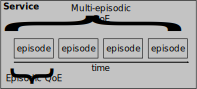
\includegraphics[width=1\columnwidth]{fig/multi-episodic}
	\caption{Repeated usage episodes with one service and their episodic QoE form a multi-episodic QoE in the user.}
	\label{img:chap01:multi-episodic}
\end{figure}

%Memory
Each usage episode has a perceived quality, which can be assessed momentary while in the usage episode and also in retrospective after the usage episode is finished.
Multi-episodic perceived quality requires experiencing multiple usage episodes with a service, but unknown how this the integration of prior experiences occurs.
It could be a continuous process that integrates current experiences immediately into a current view, a retrospective assessment evaluating all memorized and recallable information, or a mixture of both. %ist eine forwardref auf belief-adjustment model

%TODO: NAME time-frames! hour, days and also weeks.
\section{Goals}
In this thesis I pursue two goals towards understanding multi-episodic perceived quality.
In fact, the development of multi-episodic perceived quality cannot be observed directly (cf. \autoref{chap:02}) and therefore multi-episodic perceived quality can only sampled resulting in a judgment of the multi-episodic perceived quality.

\paragraph*{Goal 1}
I will investigate what affects a retrospective multi-episodic quality judgment.
The major focus here is to understand which usage episode are of special importance for a multi-episodic quality judgment to identify underlying temporal effects.

\paragraph*{Goal 2}
Second, I will investigate how multi-episodic quality can be predicted based upon episodic quality judgments.
The modeling will be based upon effects and use those to derive suiting model components.

\section{Structure}
This thesis is divided into two parts.
In \emph{Part I} I will introduce concepts and fundamentals that form the basis for my approach towards multi-episodic quality.
In \autoref{chap:02} an introduction on \ac{QoE} is given.
This includes prior work on psychophysics, perception and the quality formation process.
At the end of this chapter the relationship to higher level concepts like satisfaction and service quality is discussed.
In \autoref{chap:03} I present relevant concepts that affect recall and thus retrospective judgments of a \emph{general experience}.
Here, I will discuss how memory affects those retrospective judgments and present known temporal effects from related fields.
Based upon \autoref{chap:02} and \autoref{chap:03} I will present the state-of-the-art on performance fluctuations on QoE in one usage episode in \autoref{chap:04}.
This chapter closes with a review on found temporal effects in this domain and what how those effects are modeled.

In \emph{Part II} multi-episodic QoE is presented.
First an overview on prior work on multi-episodic QoE is given in \autoref{chap:05}.
Here the assessment methodology developed for multi-episodic QoE presented in \cite{moller_single-call_2011} is presented in detail.
This task-driven assessment method is the basis for my work and I will apply as well as extend this method further.
In \autoref{chap:06} I present my work on multi-episodic perceived quality in time-frame of up to one hour.
Those studies and the found results are then complemented in \autoref{chap:07} with studies on multi-episodic perceived quality over several days.
In \autoref{chap:08} the prediction models for multi-episodic perceived quality are implemented presened.
\autoref{chap:09} summarizes the thesis, discusses the results and highlights direction for future work.